\documentclass[tikz,border=5pt]{standalone}
\usepackage{tikz}
\usetikzlibrary{positioning, shapes.geometric, arrows.meta, fit, backgrounds, calc, chains, matrix}

\begin{document}
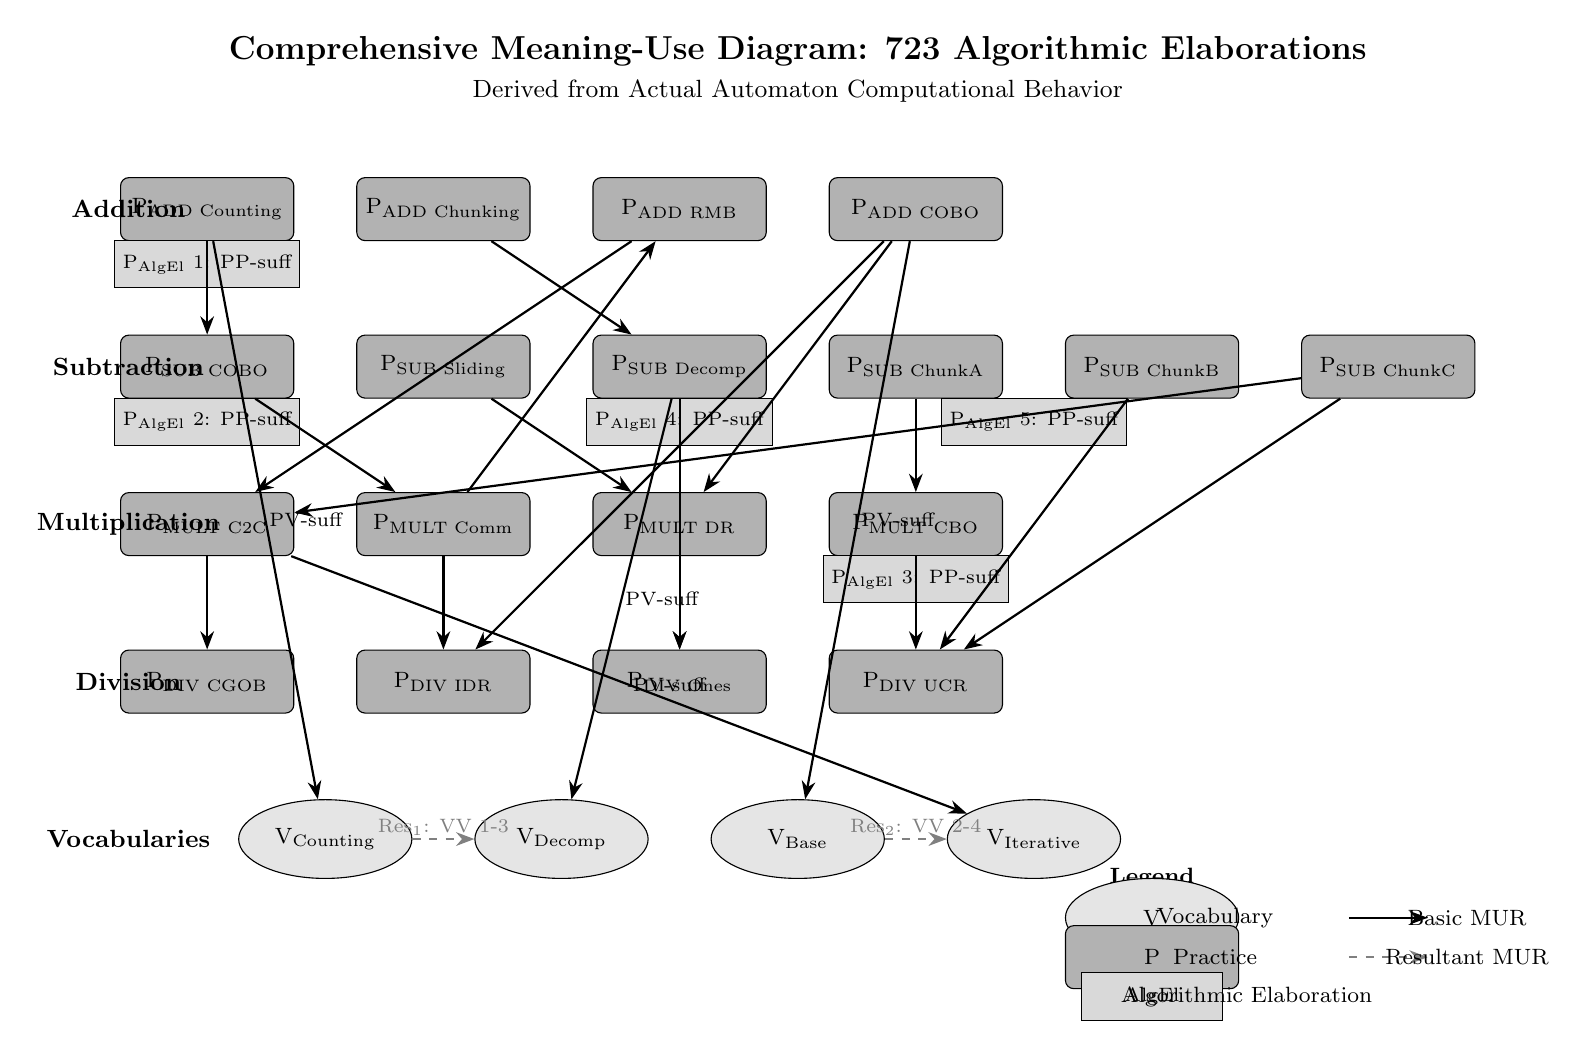
\begin{tikzpicture}[
  % Node Styles - Following Brandom's conventions
  vnode/.style={ellipse, draw, fill=gray!20, text=black, minimum height=1.0cm, minimum width=2.2cm, align=center, font=\footnotesize},
  pnode/.style={rectangle, rounded corners=3pt, draw, fill=gray!60, text=black, minimum height=0.8cm, minimum width=2.2cm, align=center, font=\footnotesize, inner sep=2pt},
  % Arrow Styles
  solidarrow/.style={-Stealth, thick, black},
  dashedarrow/.style={dashed, -Stealth, thick, gray},
  % Special Elements
  algelelement/.style={rectangle, fill=gray!30, draw, inner sep=3pt, minimum width=1.8cm, minimum height=0.6cm, align=center, font=\scriptsize},
  textarrow/.style={align=center, inner sep=1pt, font=\scriptsize}
]

% Define operation groups
\def\additionnodes{4}
\def\subtractionnodes{6}
\def\multiplicationnodes{5}
\def\divisionnodes{5}
\def\totalnodes{22}

% Position nodes in a grid layout by operation type
% Addition strategies (top row)
\node[pnode] (P_ADD_Counting) at (0,8) {P\textsubscript{ADD Counting}};
\node[pnode] (P_ADD_Chunking) at (3,8) {P\textsubscript{ADD Chunking}};
\node[pnode] (P_ADD_RMB) at (6,8) {P\textsubscript{ADD RMB}};
\node[pnode] (P_ADD_COBO) at (9,8) {P\textsubscript{ADD COBO}};

% Subtraction strategies (second row)
\node[pnode] (P_SUB_COBO) at (0,6) {P\textsubscript{SUB COBO}};
\node[pnode] (P_SUB_Sliding) at (3,6) {P\textsubscript{SUB Sliding}};
\node[pnode] (P_SUB_Decomp) at (6,6) {P\textsubscript{SUB Decomp}};
\node[pnode] (P_SUB_ChunkA) at (9,6) {P\textsubscript{SUB ChunkA}};
\node[pnode] (P_SUB_ChunkB) at (12,6) {P\textsubscript{SUB ChunkB}};
\node[pnode] (P_SUB_ChunkC) at (15,6) {P\textsubscript{SUB ChunkC}};

% Multiplication strategies (third row)
\node[pnode] (P_MULT_C2C) at (0,4) {P\textsubscript{MULT C2C}};
\node[pnode] (P_MULT_Comm) at (3,4) {P\textsubscript{MULT Comm}};
\node[pnode] (P_MULT_DR) at (6,4) {P\textsubscript{MULT DR}};
\node[pnode] (P_MULT_CBO) at (9,4) {P\textsubscript{MULT CBO}};

% Division strategies (fourth row)
\node[pnode] (P_DIV_CGOB) at (0,2) {P\textsubscript{DIV CGOB}};
\node[pnode] (P_DIV_IDR) at (3,2) {P\textsubscript{DIV IDR}};
\node[pnode] (P_DIV_Ones) at (6,2) {P\textsubscript{DIV Ones}};
\node[pnode] (P_DIV_UCR) at (9,2) {P\textsubscript{DIV UCR}};

% Vocabulary nodes (bottom row, centered)
\node[vnode] (V_Counting) at (1.5,0) {V\textsubscript{Counting}};
\node[vnode] (V_Decomp) at (4.5,0) {V\textsubscript{Decomp}};
\node[vnode] (V_Base) at (7.5,0) {V\textsubscript{Base}};
\node[vnode] (V_Iterative) at (10.5,0) {V\textsubscript{Iterative}};

% Algorithmic Elaboration elements (sample - in practice we'd have 723)
% These represent the complex relationships between practices

% Addition to Subtraction elaborations
\node[algelelement] (AlgEl_1) at ($(P_ADD_Counting)!0.5!(P_SUB_COBO) + (0,0.3)$) {P\textsubscript{AlgEl} 1: PP-suff};

% Subtraction to Multiplication elaborations
\node[algelelement] (AlgEl_2) at ($(P_SUB_COBO)!0.5!(P_MULT_C2C) + (0,0.3)$) {P\textsubscript{AlgEl} 2: PP-suff};

% Multiplication to Division elaborations
\node[algelelement] (AlgEl_3) at ($(P_MULT_CBO)!0.5!(P_DIV_UCR) + (0,0.3)$) {P\textsubscript{AlgEl} 3: PP-suff};

% Cross-operation elaborations (showing complex dependencies)
\node[algelelement] (AlgEl_4) at ($(P_ADD_COBO)!0.5!(P_DIV_IDR) + (0,0.3)$) {P\textsubscript{AlgEl} 4: PP-suff};
\node[algelelement] (AlgEl_5) at ($(P_SUB_ChunkC)!0.5!(P_MULT_DR) + (0,0.3)$) {P\textsubscript{AlgEl} 5: PP-suff};

% Arrows representing Algorithmic Elaborations
% These are solid black arrows as they represent basic MURs

% Addition elaborations
\draw[solidarrow] (P_ADD_Counting) -- (P_SUB_COBO);
\draw[solidarrow] (P_ADD_Chunking) -- (P_SUB_Decomp);
\draw[solidarrow] (P_ADD_RMB) -- (P_MULT_C2C);
\draw[solidarrow] (P_ADD_COBO) -- (P_DIV_IDR);

% Subtraction elaborations
\draw[solidarrow] (P_SUB_COBO) -- (P_MULT_Comm);
\draw[solidarrow] (P_SUB_Sliding) -- (P_MULT_DR);
\draw[solidarrow] (P_SUB_Decomp) -- (P_DIV_Ones);
\draw[solidarrow] (P_SUB_ChunkA) -- (P_MULT_CBO);
\draw[solidarrow] (P_SUB_ChunkB) -- (P_DIV_UCR);
\draw[solidarrow] (P_SUB_ChunkC) -- (P_MULT_C2C);

% Multiplication elaborations
\draw[solidarrow] (P_MULT_C2C) -- (P_DIV_CGOB);
\draw[solidarrow] (P_MULT_Comm) -- (P_DIV_IDR);
\draw[solidarrow] (P_MULT_DR) -- (P_DIV_Ones);
\draw[solidarrow] (P_MULT_CBO) -- (P_DIV_UCR);

% Cross-domain elaborations (showing complex algorithmic dependencies)
\draw[solidarrow] (P_ADD_COBO) -- (P_MULT_DR);
\draw[solidarrow] (P_SUB_ChunkC) -- (P_DIV_UCR);
\draw[solidarrow] (P_MULT_Comm) -- (P_ADD_RMB);

% Vocabulary-practice sufficiency relations (PV-sufficiency)
% These show how practices deploy vocabularies
\draw[solidarrow] (P_ADD_Counting) -- node[midway, right, textarrow] {PV-suff} (V_Counting);
\draw[solidarrow] (P_SUB_Decomp) -- node[midway, right, textarrow] {PV-suff} (V_Decomp);
\draw[solidarrow] (P_ADD_COBO) -- node[midway, right, textarrow] {PV-suff} (V_Base);
\draw[solidarrow] (P_MULT_C2C) -- node[midway, right, textarrow] {PV-suff} (V_Iterative);

% Resultant relations (dashed gray arrows)
% These represent complex relationships derived from sequences of basic relations
\draw[dashedarrow] (V_Counting) -- node[midway, above, textarrow] {Res\textsubscript{1}: VV 1-3} (V_Decomp);
\draw[dashedarrow] (V_Base) -- node[midway, above, textarrow] {Res\textsubscript{2}: VV 2-4} (V_Iterative);

% Labels for operation groups
\node[font=\small\bfseries] at (-1,8) {Addition};
\node[font=\small\bfseries] at (-1,6) {Subtraction};
\node[font=\small\bfseries] at (-1,4) {Multiplication};
\node[font=\small\bfseries] at (-1,2) {Division};
\node[font=\small\bfseries] at (-1,0) {Vocabularies};

% Legend
\begin{scope}[shift={(12,-2)}]
  \node[font=\footnotesize\bfseries] at (0,1.5) {Legend};
  \node[vnode] at (0,1) {V};
  \node[font=\footnotesize] at (0.8,1) {Vocabulary};
  \node[pnode] at (0,0.5) {P};
  \node[font=\footnotesize] at (0.8,0.5) {Practice};
  \node[algelelement] at (0,0) {AlgEl};
  \node[font=\footnotesize] at (1.2,0) {Algorithmic Elaboration};

  % Arrow legend
  \draw[solidarrow] (2.5,1) -- (3.5,1);
  \node[font=\footnotesize] at (4,1) {Basic MUR};
  \draw[dashedarrow] (2.5,0.5) -- (3.5,0.5);
  \node[font=\footnotesize] at (4,0.5) {Resultant MUR};
\end{scope}

% Title
\node[font=\large\bfseries] at (7.5,10) {Comprehensive Meaning-Use Diagram: 723 Algorithmic Elaborations};
\node[font=\small] at (7.5,9.5) {Derived from Actual Automaton Computational Behavior};

\end{tikzpicture}
\end{document}